\section{Постановка проблеми}
 
Виробники автомобілів, електроніки та телекомунікаційні компанії налаштовані на створення комп’ютерних інформаційних систем на всіх транспортних засобах. Більшість автомобілів сьогодні оснащені інтерактивними інформаційними системами, включаючи високоякісні аудіо / відео системи, супутникові навігаційні системи, гарнітури телефонії та контроль над кліматом та технічним станом автомобіля \cite{art1,Kravchenko_2009,Heisterkamp_2001}.

Незважаючи на те, що більшість систем в автомобілі є дисплеєм, голосова взаємодія стає все більш широко використовуватися в автомобільних системах. Використання голосової технології в автомобілі допомагає збільшити кількість контрольованих функцій і систем, кнопки яких не можуть бути встановлені на рульовому колесі та приладовій панелі, оскільки обмежено простір. Голосова технологія також дозволяє водіям триматися руками за кермо, а очі не відривати від дороги під час взаємодії з системою \cite{art1,Kravchenko_2009,Heisterkamp_2001}.

У зв’язку з дедалі активнішим використанням природного інтерфейсу і зокрема голосу для спілкування водія з технікою зросло і значення систем голосового управління в самому автомобілі як носія інформації у системах диспетчерського контролю за рухом автотранспорту при здійсненні етапів дистрибуції «склад – дорога – точка доставки» \cite{art1}.

Саме голосова інформація в системах диспетчерського контролю за рухом автотранспорту при взаємодії із водієм потребує формалізації у випадку проведення автоматизації таких систем.

\section{Аналіз останніх досліджень і публікацій}

Для сучасних систем голосового управління існують проблеми, пов’язані з наявністю багатьох різних розмовних мов, притаманних їм діалектів та окремих формулювань, а також з індивідуальними особливостями вимови людини і її швидкістю мови. Для цього в системах голосового управління використовують різні фільтри шумів, які прибирають зайві звуки з підвищенням якості в процесі розпізнавання команд тощо \cite{Kravchenko_2009,Heisterkamp_2001,Jonsson_2009}.

Слід зазначити, що для випадку наявності достатньо потужної системи, голосову взаємодію з водієм можна використовувати для підтримання діалогу під час руху вночі, аби не дати водію заснути \cite{Kravchenko_2012}.

Підхід, який існує для голосового управління, заснований на теорії несилової взаємодії \cite{Teslia_2010} – рефлекторна система голосового управління \cite{Egorchenkov_2016,Pylypenko_2009}. Ідея, покладена в основу цього підходу, полягає в тому, щоб замість переведення голосової інформації в текстову репрезентацію, аналізувати безпосередньо інформаційну складову сказаного, визначаючи, яку з відомих реакцій потрібно виконати.

Використання таких часткових функцій голосового управління, які підвищують комфорт водія, також повинно мати певний позитивний ефект. Проте ці функції не забезпечують оптимізації саме процесів дистрибуції.

Для формалізації голосової інформації можна використати систему з двох основних модулів: автоматичного фонетичного стенографа і ядра рефлекторної системи голосового управління (РСГУ), поточна реалізація яких визначає умови їх використання в моделі голосової взаємодії водія при диспетчерському контролі за рухом автотранспорту (рис. \ref{img:rsgu_struct}) \cite{Teslia_2014,Teslia_2013}.

Застосування алгоритму фонетичного стенографа дозволяє будувати послідовність контекстів для мовного сигналу без використання будь-якого словника. Для цієї мети будується деяка генеративна граматика, яка може синтезувати всі можливі модельні сигнали безперервної мови для будь-якої послідовності фонем. В рамках побудованої моделі будується алгоритм пофонемного розпізнавання для невідомого сигналу з використанням контекстів та можливих реакцій на них.

\section{Постановка завдання}

У даній статті необхідно запропонувати метод формалізації голосової інформації в системах диспетчерського контролю за рухом автотранспорту.

\section{Виклад основного матеріалу}

У розглядаємій системі формалізації голосової інформації (рис. \ref{img:rsgu_struct}) вхідною інформацією виступає голосова команда, яка може бути представлена звуковою хвилю; вихідною ж інформацією буде виступати процес керуючого впливу на об’єкт управління, тобто відбуватиметься виконання розпізнаної команди відповідно до попередньо заданих голосом параметрам.

Виконання фонетичного стенографу \cite{Pylypenko_2009} здійснено у вигляді бінарного додатку, набору бібліотек і конфігураційних файлів для платформи Windows, а саме ядро РСГУ виконує реалізацію інтроформаційного методу вироблення рефлексів, яке розроблено і виконане в середовищі MS Access на всіх операційних системах сімейства Windows.

Сама система формалізації голосової інформації в процесі роботи буде генерувати потрібні візуальні і голосові інформаційні повідомлення водію, це, в свою чергу, надає можливість відслідковувати процес розпізнавання команд, реакції на них і, крім того, дозволяє в реальному масштабі часу змінювати поведінку системи в разі потреби.

\begin{figure}
	\centering
	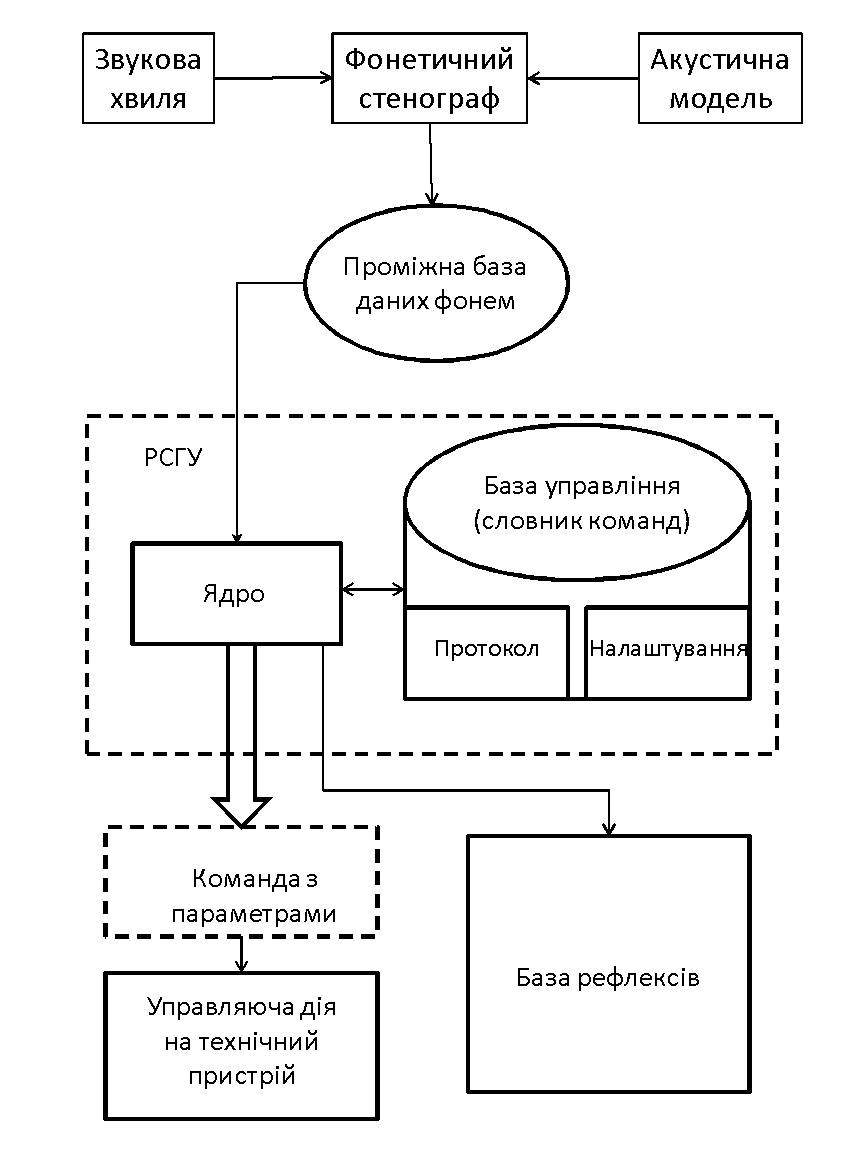
\includegraphics [width=.5\linewidth] {rsgu_struct}
	\caption{Структура системи формалізації голосової інформації в моделі голосової взаємодії водія при диспетчерському контролі за рухом автотранспорту}
	\label{img:rsgu_struct}
\end{figure}

Розглянемо схему роботи системи формалізації голосової інформації в моделі голосової взаємодії водія при диспетчерському контролі за рухом автотранспорту. Водій у вільній формі озвучує необхідні для нього дії системи. Наприклад, по відношенню до голосового управління системою: «Показати маршрутний лист», або «Показати мапу маршруту», або «Показати інформацію про точку». Програмна платформа системи формалізації голосової інформації в моделі голосової взаємодії водія при диспетчерському контролі за рухом автотранспорту передає необхідну команду на технічний пристрій, або озвучує водієві інформацію, затребувану в його команді. При навчанні водій сам виконує відповідну дію, і у системи виробляється рефлекс на подібне звернення. Якщо водій (чи інший водій, який закріплений на автотранспортному засобі) говорить «по-різному», то виробляється стійкий рефлекс саме на інформативну частину голосової команди.

При цьому в системі формалізації голосової інформації в моделі голосової взаємодії водія при диспетчерському контролі за рухом автотранспорту наявні наступні стани, команди та засоби:

1. \textbf{Звукова команда}. Водій голосом звертається з проханням до технічного пристрою.

Вихідною інформацією є звукова хвиля.

Наведемо приклад для даної команди: покажи мені, будь ласка, інформацію про точку;

2. \textbf{Акустична модель}. Включає статистичний опис розпізнаваємої мови і особливостей мови водія. Статистичний опис формується в процесі навчання налаштуванням на водіїв. У якості акустичних моделей використовуються приховані Марківські моделі. 65 українських контекстно-незалежних фонем моделюються трьома станами Марківського ланцюга без пропуску.

Створення словника транскрипцій акустичних моделей відбувається автоматично з орфографічного словника з використанням контекстно-незалежних правил;

3. \textbf{Фонетичний стенограф}. Служить для перетворення вхідного оцифрованого звукового сигналу, що містить усне мовлення (акустичної моделі), в набір фонем.

Алгоритм фонетичного стенографа дозволяє будувати послідовність фонем для мовного сигналу без використання будь-якого словника. Для цієї мети будується деяка генеративна граматика, яка може синтезувати всі можливі модельні сигнали безперервної мови для будь-якої послідовності фонем. В рамках побудованої моделі будується алгоритм пофонемного розпізнавання для невідомого сигналу. Використовуються ті ж контекстнонезалежні моделі фонем, як і в базовому розпізнавачі. Надійність виявлення фонеми на правильному місці для відомої реалізації дорівнює приблизно 70\%. Вихідна інформація: проміжна база даних фонем – результат розпізнавання вхідних звукових хвиль;

4. \textbf{Ядро РСГУ}. Призначено для моделювання системи голосового управління технічним пристроєм. Містить програмну реалізацію інтроформаційного методу, а також алгоритмів виділення комбінацій фонем і навчання (накопичення статистики). Інформаційна база управління містить словник команд, протокол роботи, налаштування системи;

5. \textbf{Команда з параметрами}. Результатом її роботи є команда з параметрами, яку необхідно реалізувати технічному пристрої.

Вихідною інформацією є виконувана команда.

Приклад: водій – Найдьонов, команда – Х хвилин, рівень – десятки, десятки хвилин – 10, одиниці хвилин – 8;

6. \textbf{Керуючий вплив}. Містить програмну реалізацію алгоритму управління технічним пристроєм.

Вхідною інформацією є перетворена у вигляд формули, команда з відповідними параметрами. Результатом керуючого впливу є зміна параметрів самого технічного пристрою. Прикладом керуючого пристрою може бути інформація про наступний час виконання. Система формалізації голосової інформації в моделі голосової взаємодії водія при диспетчерському контролі за рухом автотранспорту є простою і, у даному випадку, реалізує рефлекторну модель поведінки, що приведена на рис. \ref{img:rsgu_scheme}

Система формалізації голосової інформації в моделі голосової взаємодії водія при диспетчерському контролі за рухом автотранспорту функціонує в режимі навчання і режимі управління. У першому випадку у режимі навчання відбувається формування бази рефлексів.

У режимі управління РСГУ відбувається вироблення реакції на звернення водія. Також у цьому режимі відбувається реалізація режиму самонавчання – для випадку, коли отримана реакція не задовольняє водія.

Основною частиною системи формалізації голосової інформації в моделі голосової взаємодії водія при диспетчерському контролі за рухом автотранспорту є база рефлексів. База рефлексів містить статистику вхідних впливів (комбінацій фонем) і реакцій системи, розділених на класи: водій, команда, рівень числа, десятки, одиниці.

\begin{figure}
	\centering
	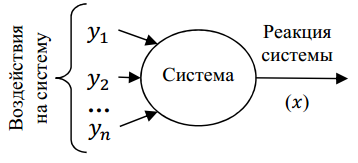
\includegraphics [width=.5\linewidth] {rsgu_scheme}
	\caption{Схема реакції системи формалізації голосової інформації в моделі голосової взаємодії водія при диспетчерському контролі за рухом автотранспорту на несилові впливи}
	\label{img:rsgu_scheme}
\end{figure}

Реалізація кожного класу рефлексів відбувається в кожному окремому компоненті системи формалізації голосової інформації в моделі голосової взаємодії водія при диспетчерському контролі за рухом автотранспорту. Представлення кожного компоненту системи здійснюється у вигляді окремого «інтроформаційного» нейрона.

На вході системи задається повний вхідний набір фонем, та/або реакція інших «інтроформаційних» нейронів, на виході – вироблена реакція нейронів, яка надходить на інші «інтроформаційні» нейрони, або на самий технічний пристрій.

У кожному компоненті системи формалізації голосової інформації в моделі голосової взаємодії водія при диспетчерському контролі за рухом автотранспорту інформація зберігається в наступних таблицях:

\begin{itemize}
	\item S – таблиця з комбінацією фонем, в якій знаходяться та зберігаються всі комбінації послідовних фонем з довжинами від 2-х до 10 символів з інформацією про те, скільки разів вони зустрічалися;
	\item R – таблиця реакції РСГУ, в якій міститься перелік дій, що необхідно виконати РСГУ або технічному пристрою, частота користування і визначеність даної реакції. Реакція типу «Не знаю» забезпечує відкритість системи;
	\item А – таблиця, що призначена для встановлення зв’язку вищенаведених таблиць S і R. Дана таблиця вміщує інформацію про те, скільки разів і яка реакція була затребувана в разі, коли на вході був деякий набір фонем. Крім того, дана таблиця містить відомості про визначеність реакції, що пов’язана з цим набором фонем.
\end{itemize}

У вищенаведених таблицях для випадку режиму навчання відбувається накопичення інформації про зв’язок вхідних фраз (контекстів) і реакцій системи формалізації голосової інформації в моделі голосової взаємодії водія при диспетчерському контролі за рухом автотранспорту. У процесі роботи системи отримана інформація використовується далі в режимі управління для вироблення реакцій на відповідні звернення водія на основі інтроформаційного методу \cite{Teslia_2010}. При цьому алгоритм реалізації режиму управління в системі має наступну послідовність:

\begin{itemize}
	\item перший етап. Старт алгоритму.
\end{itemize}

При надходженні на вхід системи потоку фонем виділяються фрагменти (набори), множиною M, що містять від 2 до 10 поруч стоячих символів;

\begin{itemize}
	\item другий етап. Відбір класу команд.
\end{itemize}

З таблиці S відбувається здійснення відбору записів, які відповідають сформованим наборам фонем, що належать до множини M.
На основі інтроформаційного методу відбувається обчислення визначеності реакцій (команд), що містяться в таблицях A і R. Команда, що має найбільшу визначеність, вибирається для реалізації;

\begin{itemize}
	\item третій етап. Якщо в команді є звернення до числового значення (знак \#), розглядаються класи рівень числа, десятки, одиниці.
\end{itemize}

Клас рівня числа. У таблиці S здійснюється відбір записів, які відповідають сформованим наборам фонем (що входять у множину M). Використовуючи таблиці A і R, відповідно до інтроформаційного методу обчислюється визначеність рівня числа. Варіанти: немає десятків хвилин (числа від 0 до 9), є десятки хвилин (числа більше 9).

Якщо рівень числа «Є десятки хвилин», то активізуються таблиці, що входять в клас десятків хвилин. У таблиці S здійснюється відбір записів, які відповідають сформованим наборам фонем (що входять в множину M). Використовуючи таблиці A і R, відповідно до інтроформаційного методу обчислюється визначеність номера десятка. Якщо десяток не визначений, в команду вставляється знак «?».

Клас одиниць хвилин. У таблиці S здійснюється відбір записів, які відповідають сформованим наборам фонем (що входять в множину M). Використовуючи таблиці A і R, відповідно до інтроформаційного методу обчислюється визначеність другий цифри в числі. Якщо цифра не визначена, в команду вставляється знак «?»;

\begin{itemize}
	\item четвертий етап. Завершення алгоритму.
\end{itemize}

Таким чином, в кожен компонент системи надходить весь вхідний набір фонем. Без виділення слів, команд, пропозицій тощо. Результат даного методу такий самий як і у головного мозку людини. Тобто, слухаючи усне мовлення, або читаючи лист, мозок, не розпізнаючи букви і слова, розпізнає сенс. Теж саме відбувається і в рефлекторній системі голосового управління. При цьому, не потрібно створювати ніяких словників, виконувати морфологічний, синтаксичний, семантичний аналіз тексту, а також виділяти слова і команди; виникнення реакції відбувається на звуковий потік, з якого система формалізації голосової інформації в моделі голосової взаємодії водія при диспетчерському контролі за рухом автотранспорту, як і людина сама «вміє виділяти» інформативну частину за максимальною визначеністю \cite{Teslia_2013}.

\section{Висновки}

У роботі запропоновано метод формалізації голосової інформації в системах диспетчерського контролю за рухом автотранспорту. Для формалізації голосової інформації запропоновано використання системи, що складається з двох основних модулів: автоматичного фонетичного стенографа і ядра рефлекторної системи голосового управління, поточна реалізація яких визначає умови їх використання в моделі голосової взаємодії. При використанні такої системи непотрібно створювати ніяких словників, виконувати морфологічний, синтаксичний, семантичний аналіз тексту, а також виділяти слова і команди; виникнення реакції відбувається на звуковий потік, з якого система формалізації голосової інформації в моделі голосової взаємодії водія при диспетчерському контролі за рухом автотранспорту, як і людина сама «вміє виділяти» інформативну частину за максимальною визначеністю.
